\begin{figure*}[t]
\centering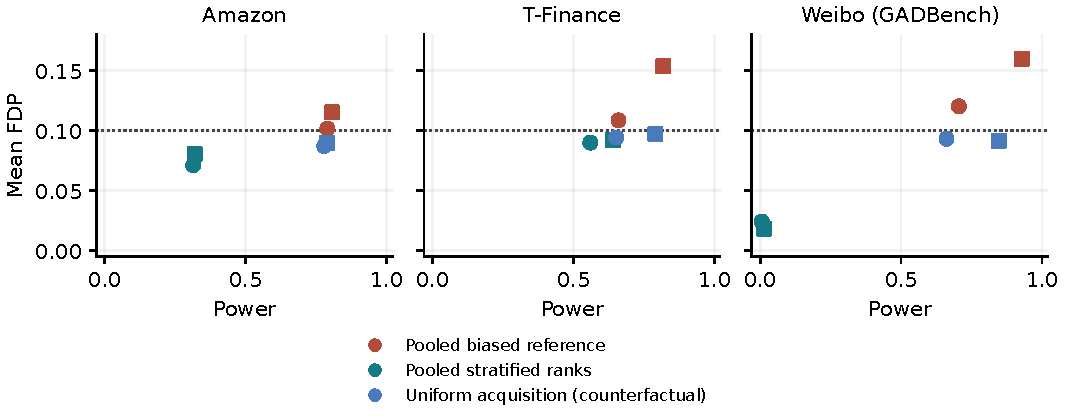
\includegraphics[width=\textwidth]{acquisition_main.pdf}
\caption{Correction can reduce FDP while sacrificing useful discoveries. Training labels define the 80/20 exposure strata; acquisition probabilities are $0.50$ and $0.10$ in the lower and upper strata. Circles denote attribute scorers and squares graph-feature scorers. All three graphs are shown, including Weibo's nearly powerless stratified result. The blue reference is a counterfactual uniform-acquisition design at comparable expected label cost, not an available reference in the biased scenario. Points average ten seed means; the dotted line marks nominal $0.10$. Figure~\ref{fig:allocationfull} and Appendix~\ref{app:allocation} retain every allocation, weighting and acquisition-severity comparison.}
\label{fig:allocation}
\end{figure*}
